\chapter{Programmbeschreibung}\label{ch:programmbeschreibung}

\section{UML-Diagramme}\label{sec:uml}

\begin{figure}[htb]
    \centering
    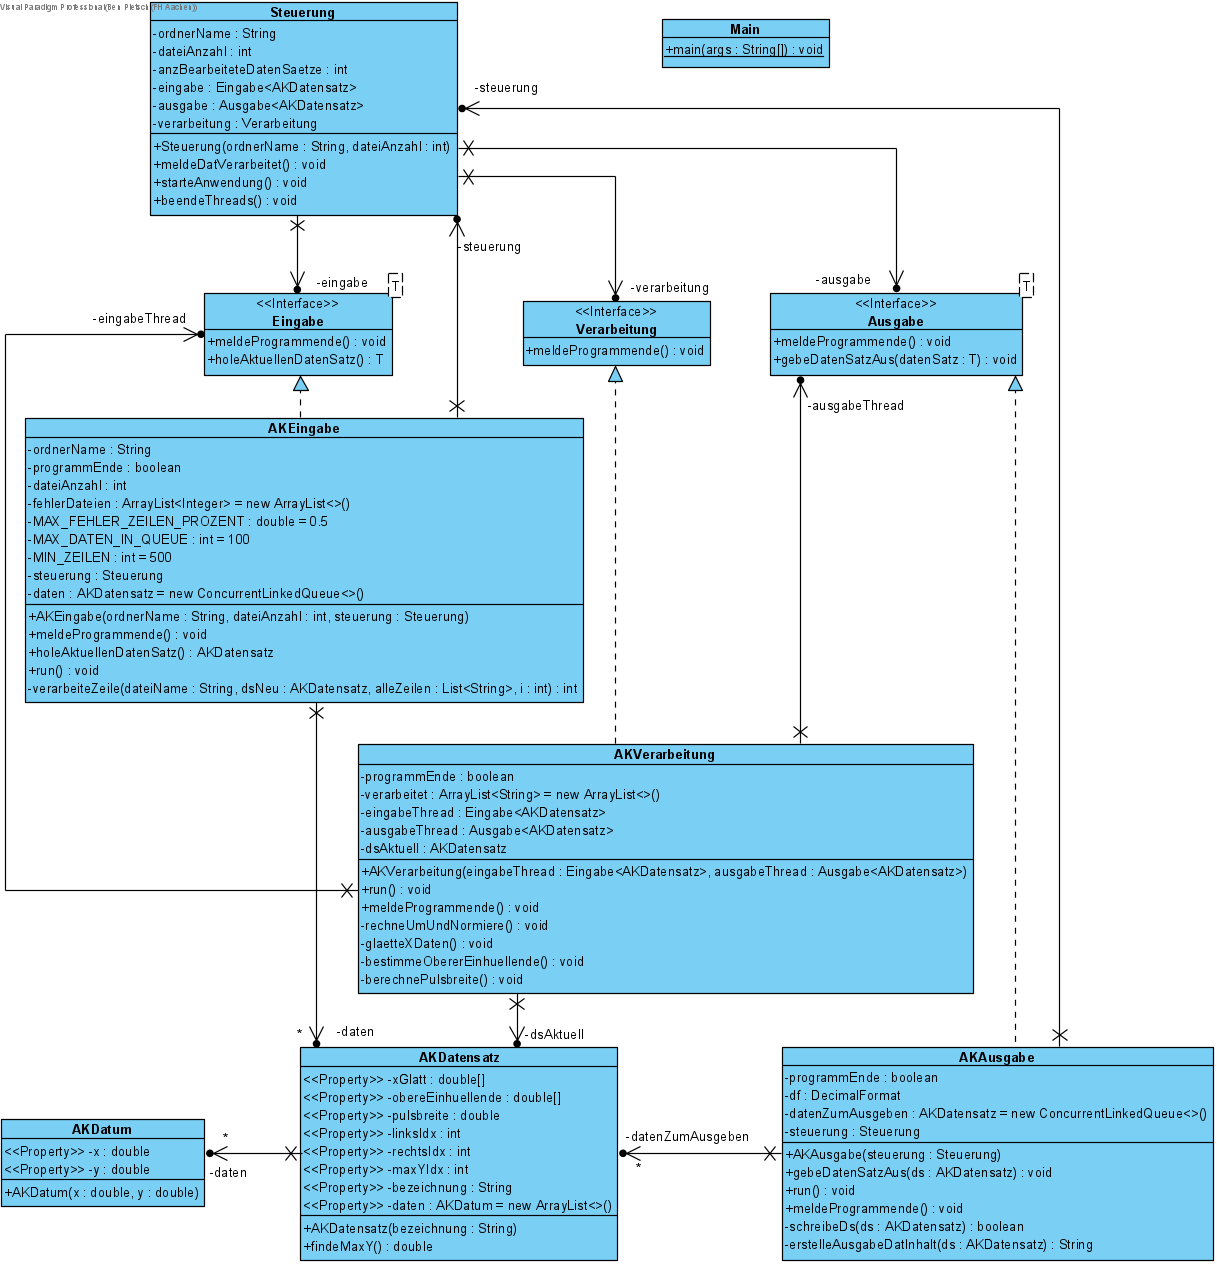
\includegraphics[width=\linewidth]{images/ClassDiagram1}
    \caption{
        Klassendiagramm.
    }
    \label{fig:klassen-dia}
\end{figure}

\section{Struktogramme}\label{sec:strukto}

\begin{figure}[htb]
    \centering
    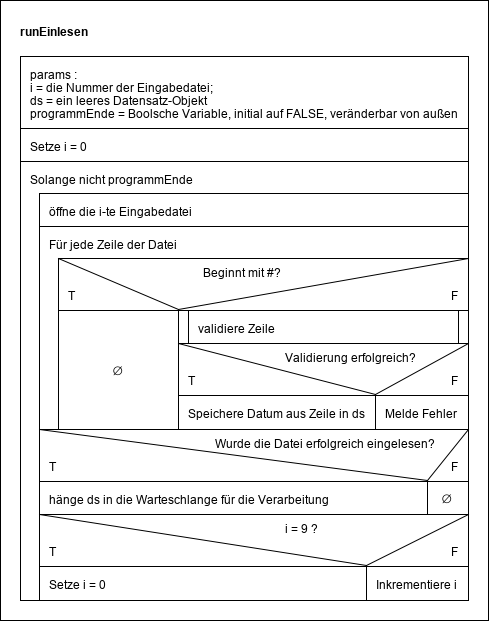
\includegraphics[width=0.8\linewidth]{images/runEinlesen}
    \caption{
        Vorgehen beim Einlesen der Textdateien.
    }
    \label{fig:run-einlesen}
\end{figure}

\begin{figure}[htb]
    \centering
    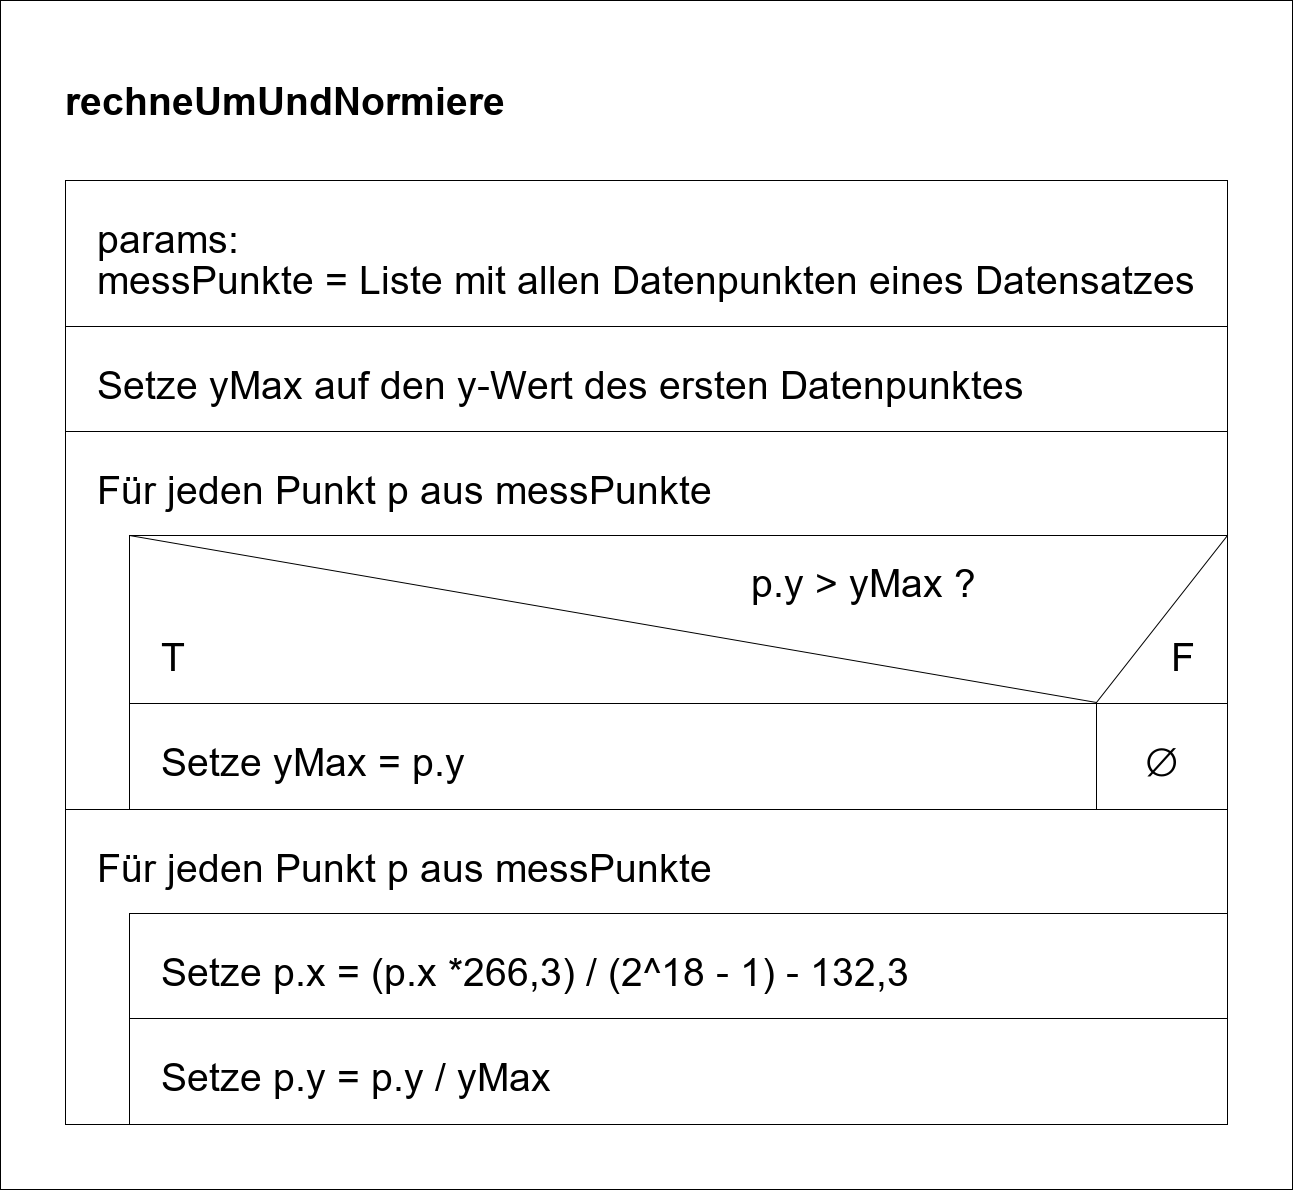
\includegraphics[width=0.7\linewidth]{images/rechneUmUndNormiere}
    \caption{
        Erster Schritt aus der Verarbeitung, siehe Abschnitt~\ref{subsec:umrechnung-und-normierung}.
    }
    \label{fig:umrechnung-normierung}
\end{figure}
\begin{figure}[htb]
    \centering
    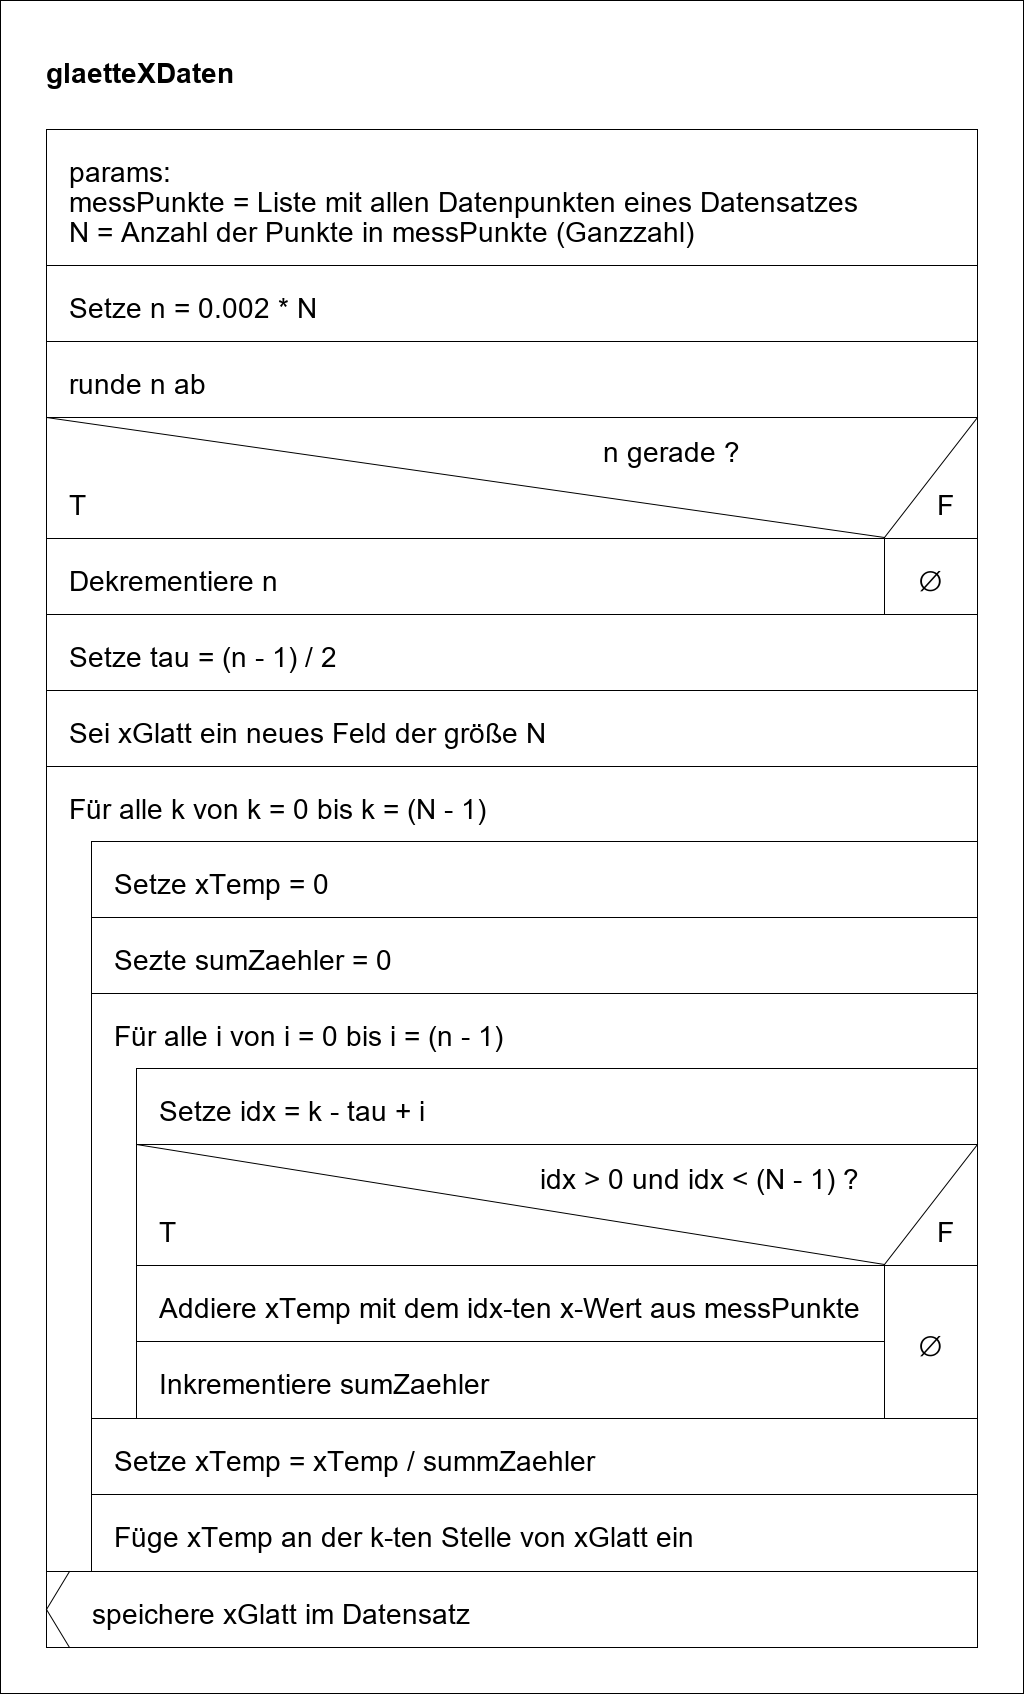
\includegraphics[width=0.7\linewidth]{images/glaetteXDaten}
    \caption{
        Zweiter Schritt der Verarbeitung, siehe Abschnitt~\ref{subsec:glaettung}.
    }
    \label{fig:glaettung-fig}
\end{figure}

\begin{figure}[htb]
    \centering
    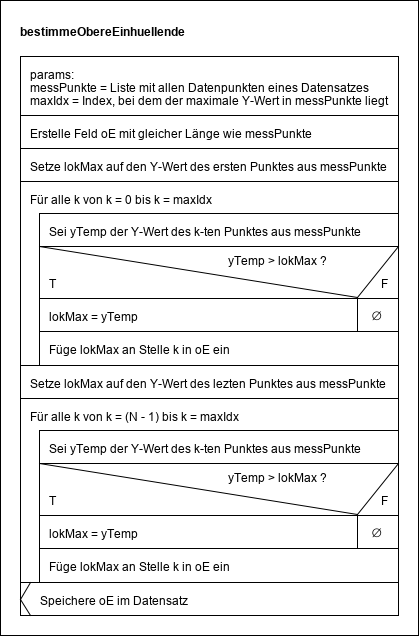
\includegraphics[width=0.7\linewidth]{images/bestimmeObereEinhuellende}
    \caption{
        Dritter Schritt der Verarbeitung, siehe Abschnitt~\ref{subsec:ober-einh}.
    }
    \label{fig:obere-ein-strukto}
\end{figure}

\begin{figure}[htb]
    \centering
    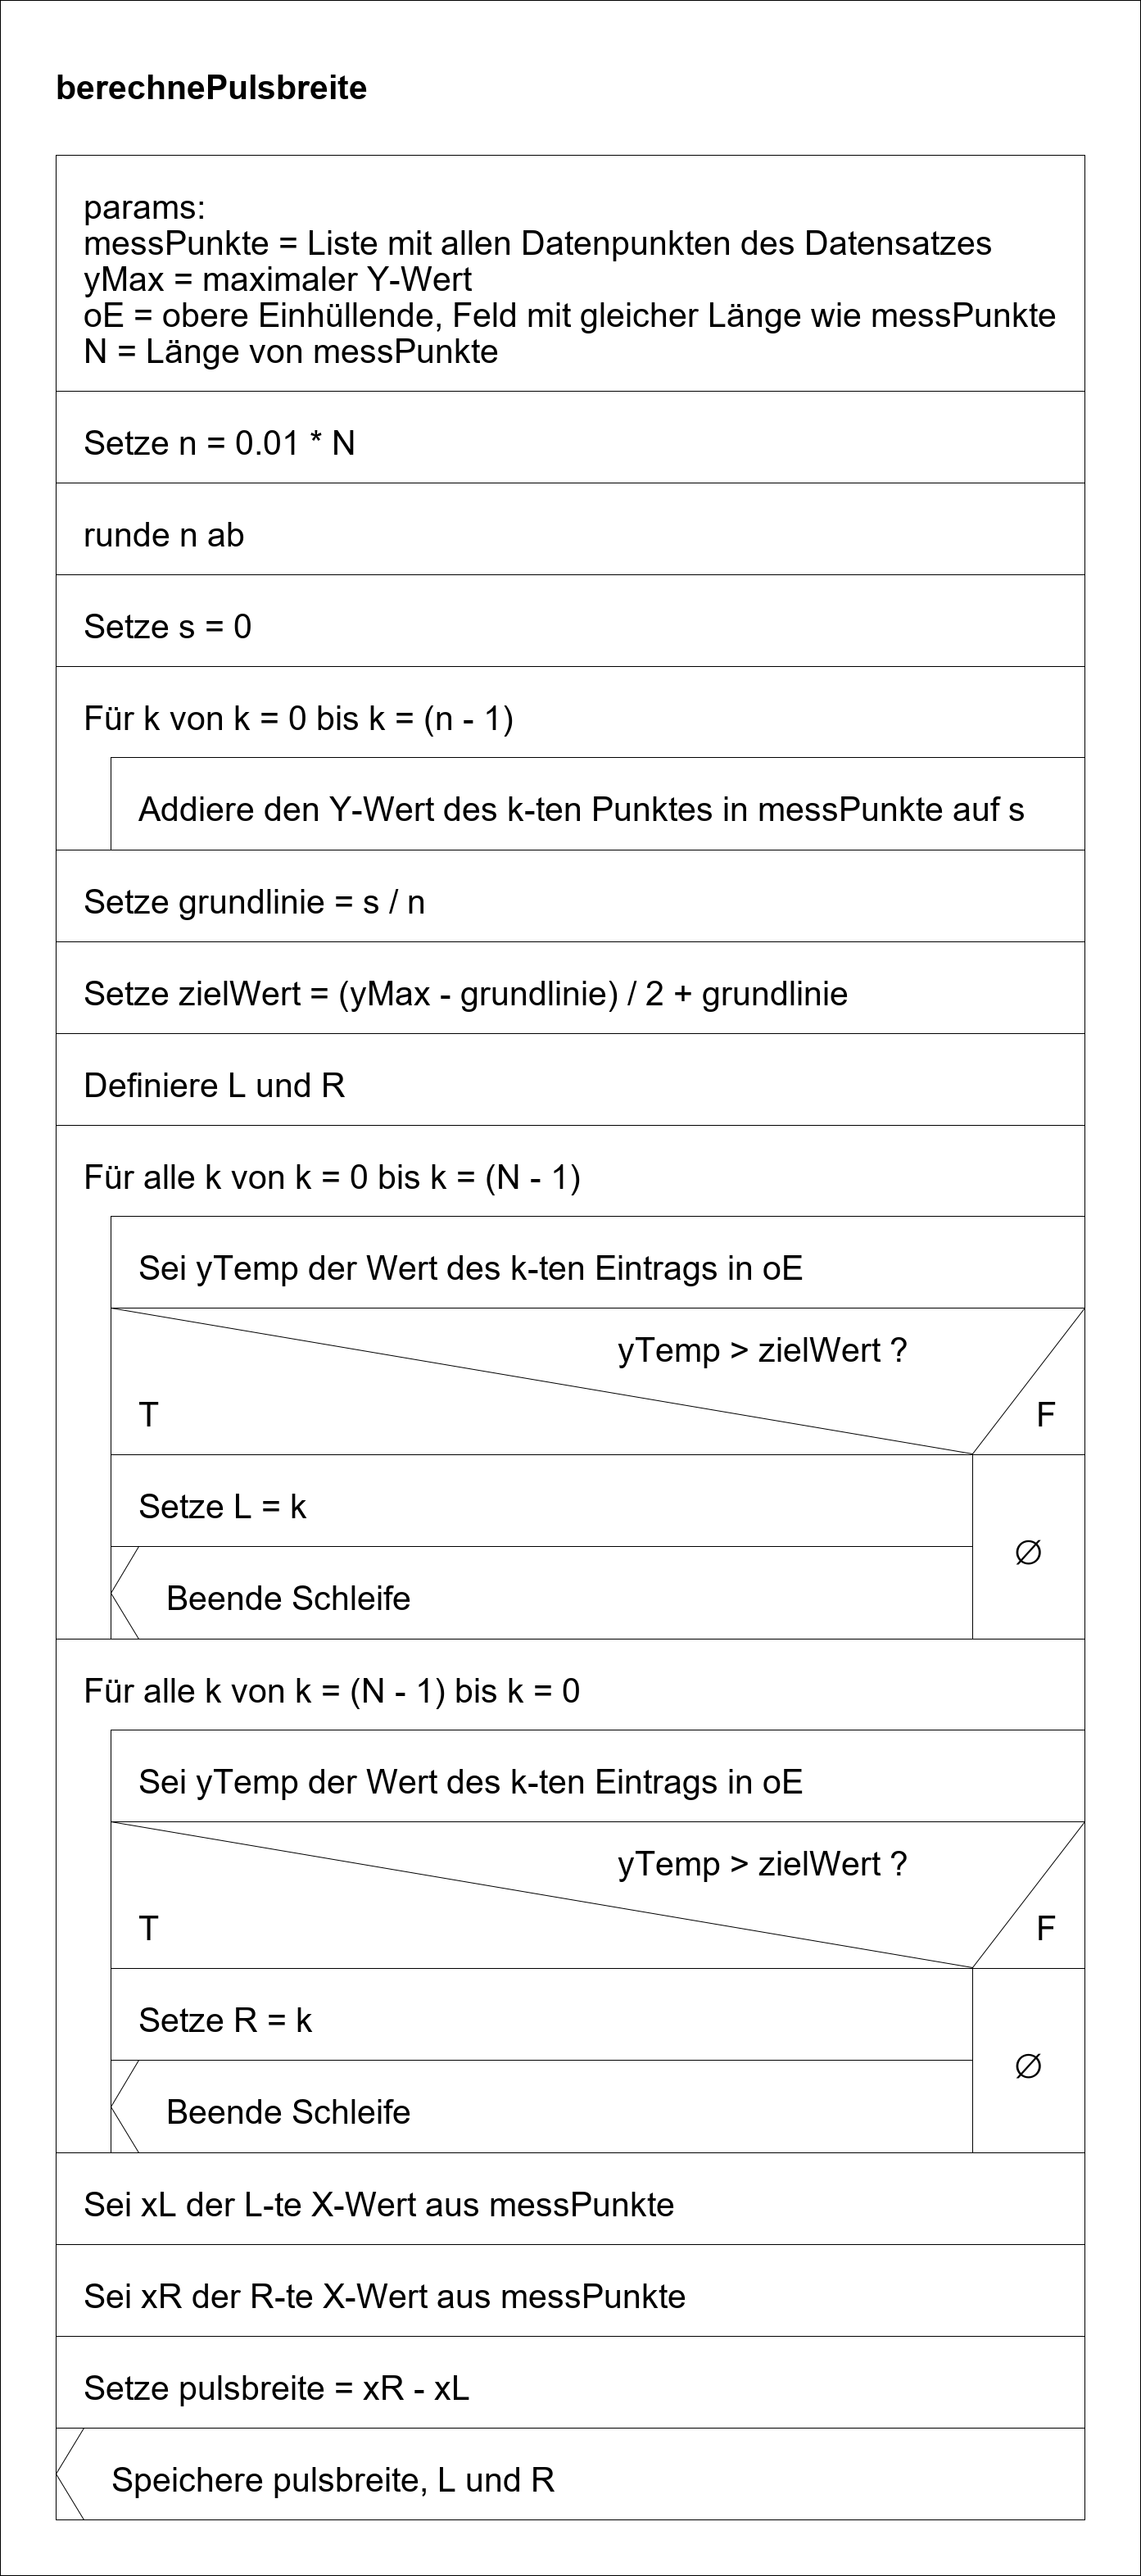
\includegraphics[width=0.7\linewidth]{images/berechnePulsbreite}
    \caption{
        Vierter Schritt der Verarbeitung, siehe Abschnitt~\ref{subsec:pulsbreite}.
    }
    \label{fig:puls-strukto}
\end{figure}

\section{Entwicklungsdokumentation}\label{sec:entwicklerdokumentation}
Im Abgabe-Ordner befindet sich ein Verzeichnis mit dem Namen \glqq JavaDoc\grqq{}.
Mit einem Doppelklick auf die darin enthaltene Datei \glqq index.html\grqq{} öffnet sich die Dokumentation im Web-Browser.